\documentclass[a4paper, amsfonts, amssymb, amsmath, reprint, showkeys, nofootinbib, twoside]{revtex4-1}
\usepackage[english]{babel}
\usepackage[utf8]{inputenc}
\usepackage[colorinlistoftodos, color=green!40, prependcaption]{todonotes}
\usepackage[pdftex, pdftitle={Article}, pdfauthor={Author}]{hyperref}
\usepackage{amsthm}
\usepackage{mathtools}
\usepackage{physics}
\usepackage{xcolor}
\usepackage{caption}
\usepackage{hyperref}
%\hypersetup{colorlinks=true, linkcolor=blue, urlcolor = blue}
\usepackage{amsmath}
\usepackage{amssymb}
\usepackage{booktabs}
\usepackage{graphicx}
\graphicspath{Images}
\usepackage[left=23mm,right=13mm,top=35mm,columnsep=15pt]{geometry} 
\usepackage{adjustbox}
\usepackage{placeins}
\usepackage[T1]{fontenc}
\usepackage{float}
\usepackage{multirow}
\usepackage{csquotes}
\usepackage{refstyle}
\usepackage{lipsum}

\begin{document}

\title{Study of Zeeman effect}
\author{Swaroop Ramakant Avarsekar}
\email{swaroop.avarsekar@niser.ac.in}
\affiliation{School of Physical Sciences, National Institute of Science Education and Research, HBNI, Jatni -752050, India}
\date{\today}
	
\maketitle

\section{Introduction and Theory}
Zeeman effect is splitting of spectral lines under time independent magnetic field, due to interaction between the magnetic field and the spin angular momentum of the electrons where each of the electrons has its spin. When magnetic field is introduced, the degeneracy is broken and transition lines are now split so that there is more lines in emission spectra, which can be visualised by Fabry Perot's etalon resulting in circular fringes. The lines split in the pattern indicates Zeeman effect.

\begin{figure}[H] %  figure placement: here, top, bottom, or page
	\centering
	\includegraphics[width=8.3cm,height=6cm]{t} 
	\caption{Splitting of components in magnetic field}
\end{figure}

If r is the radius of the lines, then
\begin{equation}
	r^2_{p+1}-r^2_p=2f^2/n_o=constant
\end{equation}
This implies that
\begin{equation}
	\Delta^{p+1,p}_a=r^2_{p+1,a}-r^2_p,a =\Delta^{p+1,p}_b=r^2_{p+1,b}-r^2_p,b
\end{equation}

\begin{equation}
	\therefore \Delta^{p+1,p}_a=\Delta^{p+1,p}_b
\end{equation}

\begin{equation}
	\delta^{p+1,p}_{a,b}=r^2_{p+1,a}-r^2_{p+1,b}
\end{equation}

\begin{equation}
	\Delta bar{\nu}=\delta/(2t\Delta)
\end{equation}
 where t is the distance between etalon plates.
 
 The energy difference to calculate Bohr's magneton is as follows,
 \begin{equation}
 	\Delta E=E_{L,M_L}-E_{L-1,M_{L-1}}=hc\Delta\bar{\nu}/2
 \end{equation}

$\Delta E$ is proportional to the magnetic field as
\begin{equation}
	\Delta E=\mu_BB
\end{equation}
 where $\mu_B$ is Bohr's magneton=$9.27\times10^{-4} J/T$
 
 \begin{equation}
\mu_B=hc\bar{\nu}/2/B
 \end{equation}

$\mu_B$ can be obtained by linear fit between $\bar{\nu}$ and B with 

\section{Experiment}
\subsection{Apparatus}
\begin{figure}[H] %  figure placement: here, top, bottom, or page
	\centering
	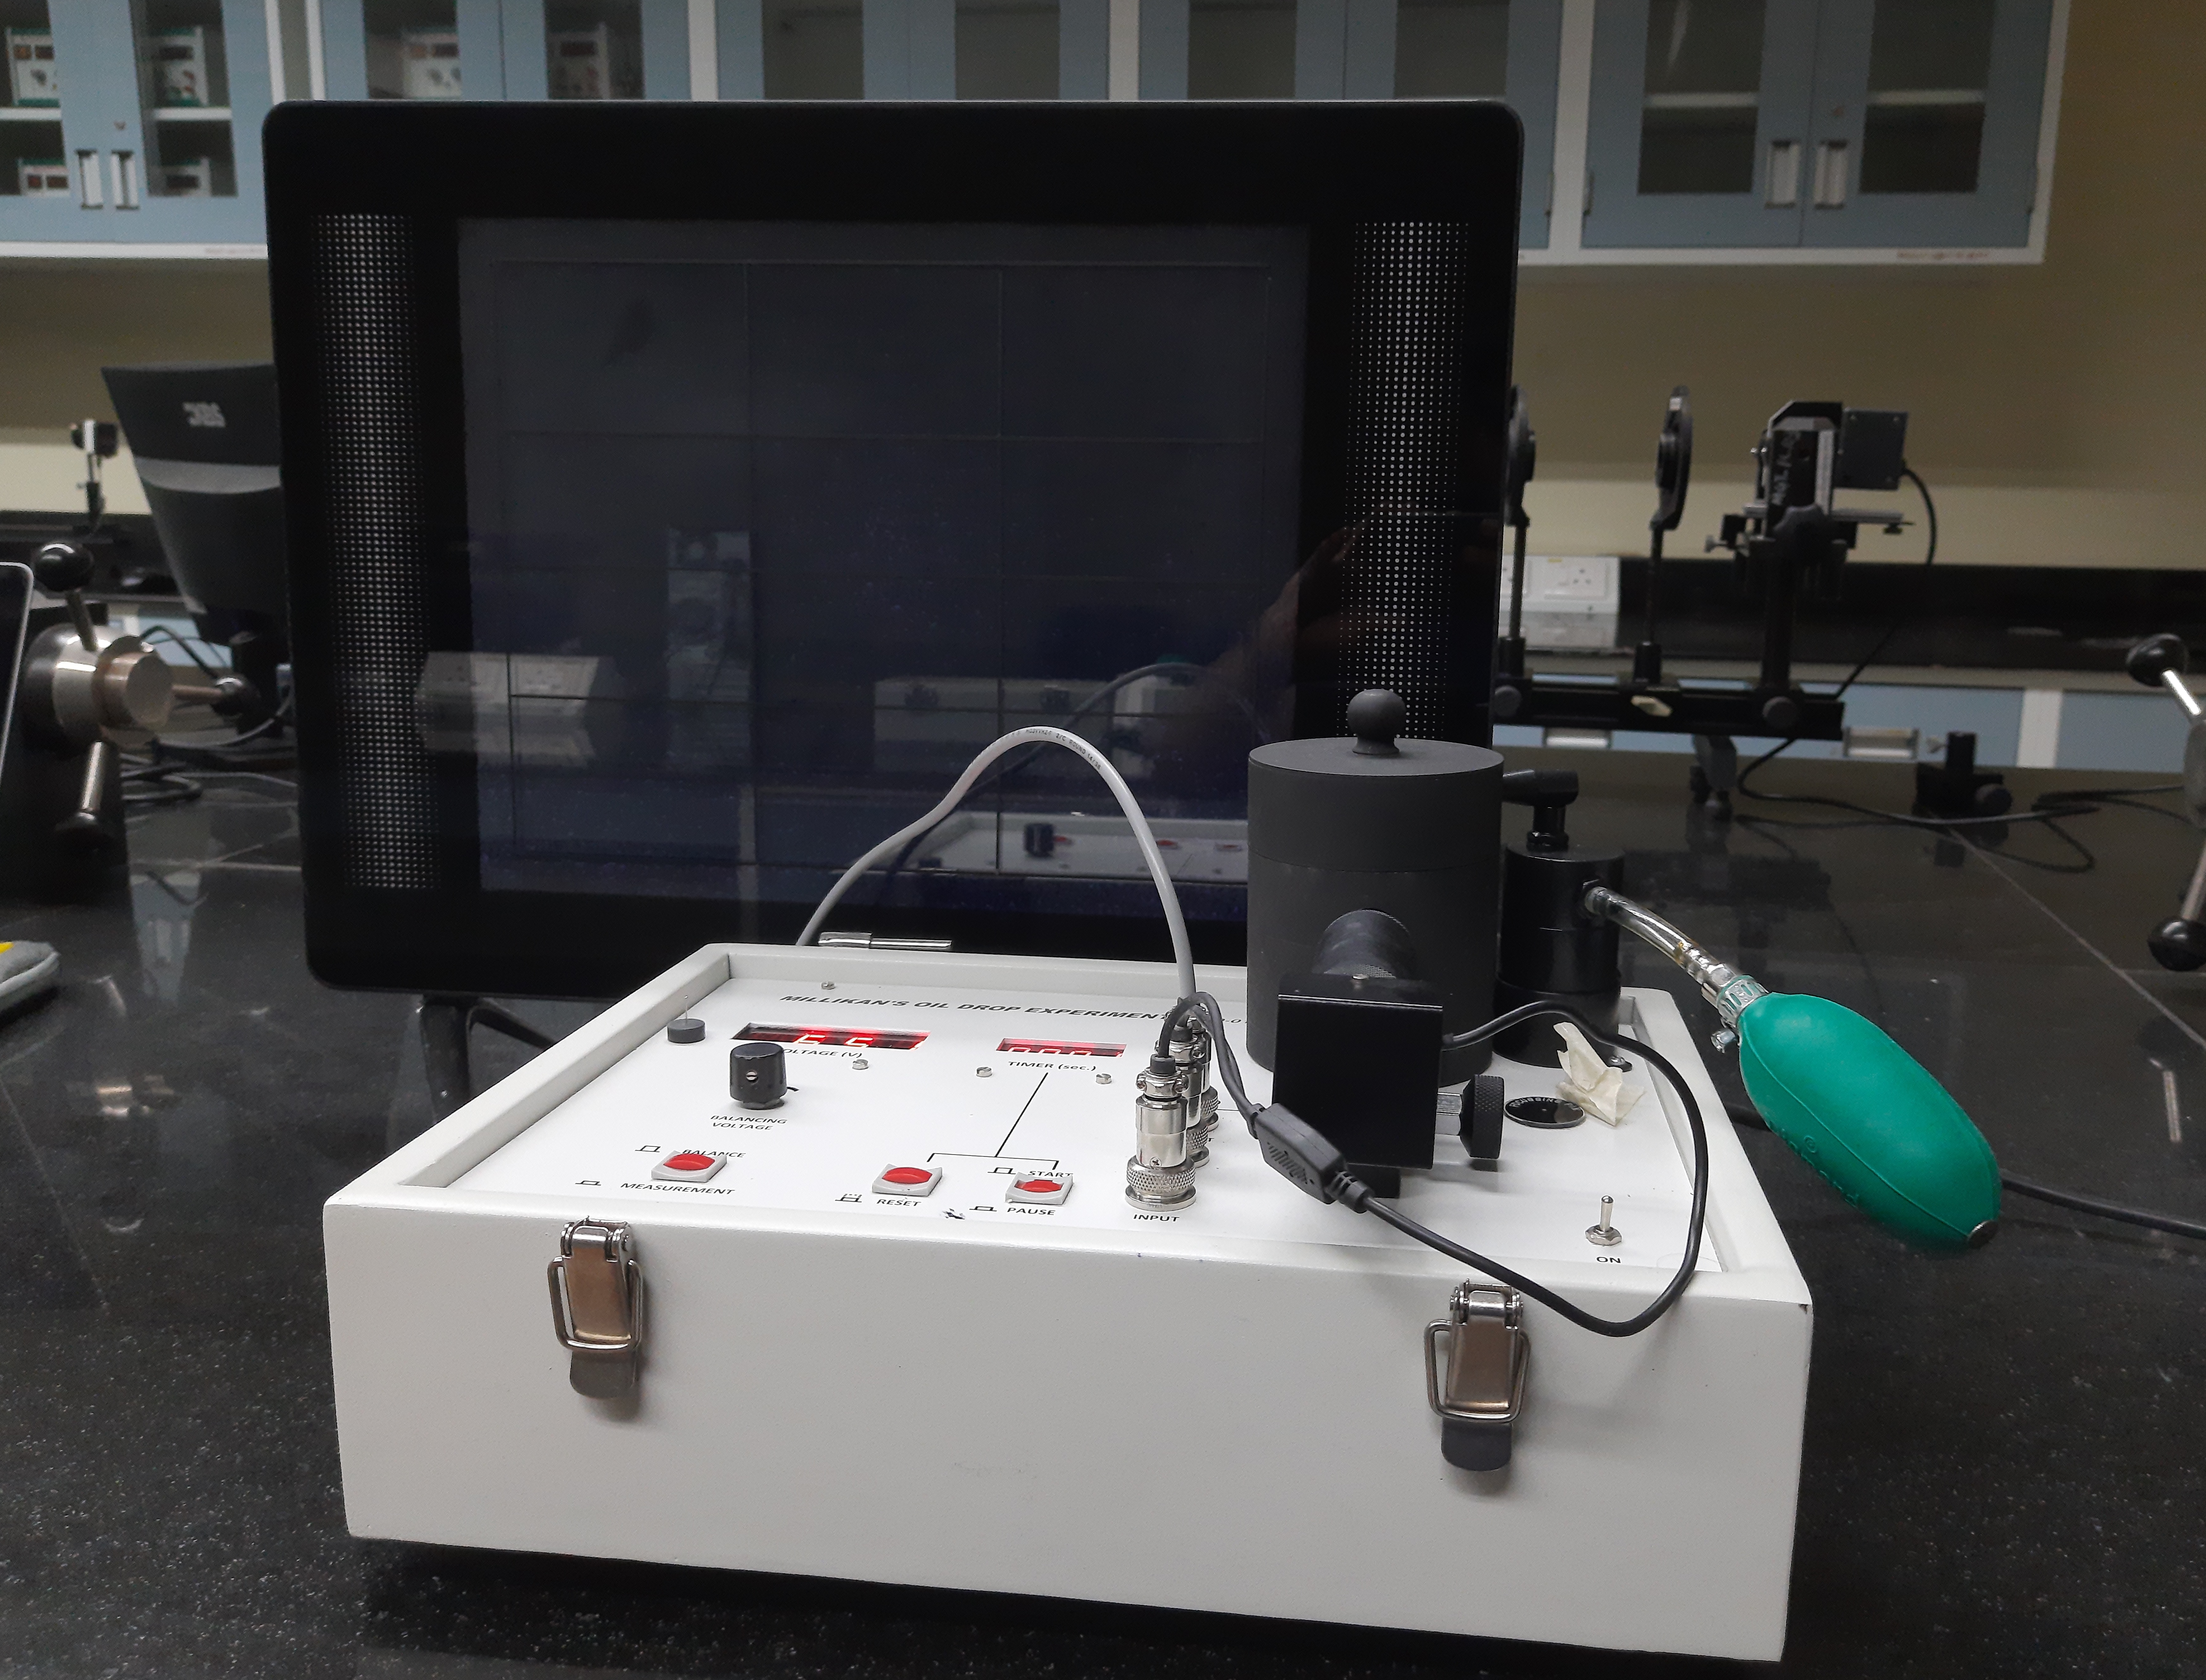
\includegraphics[width=8.3cm,height=4cm]{1} 
	\caption{Schematic diagram for experimental setup}
	\label{5}
\end{figure}

We would require Fabry-Perót etalon, permanent magnets, Cd lamp, optical bench, two lenses with f=50 mm and 300 mm, slide mounts, iris diaphragm to control amount of light, polarizing filter, CMOS camera with holder and a computer with respective software installed on it.

\subsection{Procedure}
Turn on the Cadmium light source which is placed between permanent pole pieces. The permanent magnets should be calibrated with variation of magnetic field by changing the distance between pole pieces. Align the etalon, lenses and camera such that a clear image is obtained from the computer screen. With varying the magnetic field the radius of lines varies. With the magnetic field turned on in the absence of the analyser three lines can be seen simultaneously in the normal Zeeman effect in transversal observation. In the case of the anomalous Zeeman effect three groups of three lines appear. Inserting the analyser in the normal Zeeman effect two $\sigma$ -lines can be observed if the analyser is in the vertical position, while only the $\pi$ -line appears if the analyser is turned into its horizontal position(transversal Zeeman effect). In the anomalous Zeeman effect there are two groups of three $\sigma$-lines in vertical polarization and one group of three $\pi$-lines in horizontal polarization. Turning the magnetic system by 90 degrees the light coming from the spectral lamp parallel to the direction of the field (longitudinal) can also be studied through the holes in the pole pieces. It can be shown that this light is circular polarized light (longitudinal Zeeman effect). A $\lambda$/4 -plate is generally used to convert linear into elliptical polarized light. In this experiment the plate is used in the opposite way. With the $\lambda$/4-plate inserted before the analyser, the light of the longitudinal Zeeman effect is investigated. If the optical axis of the $\lambda$/4-plate coincides with the vertical, it is observed that some rings disappear if the analyser is at an angle of +45 degrees with the vertical while other rings disappear for a position of -45 degrees . That means that the light of the longitudinal Zeeman effect is polarized in a circular (opposed way). The $\pi$-lines are longitudinally not observable.

\begin{figure}[H] %  figure placement: here, top, bottom, or page
	\centering
	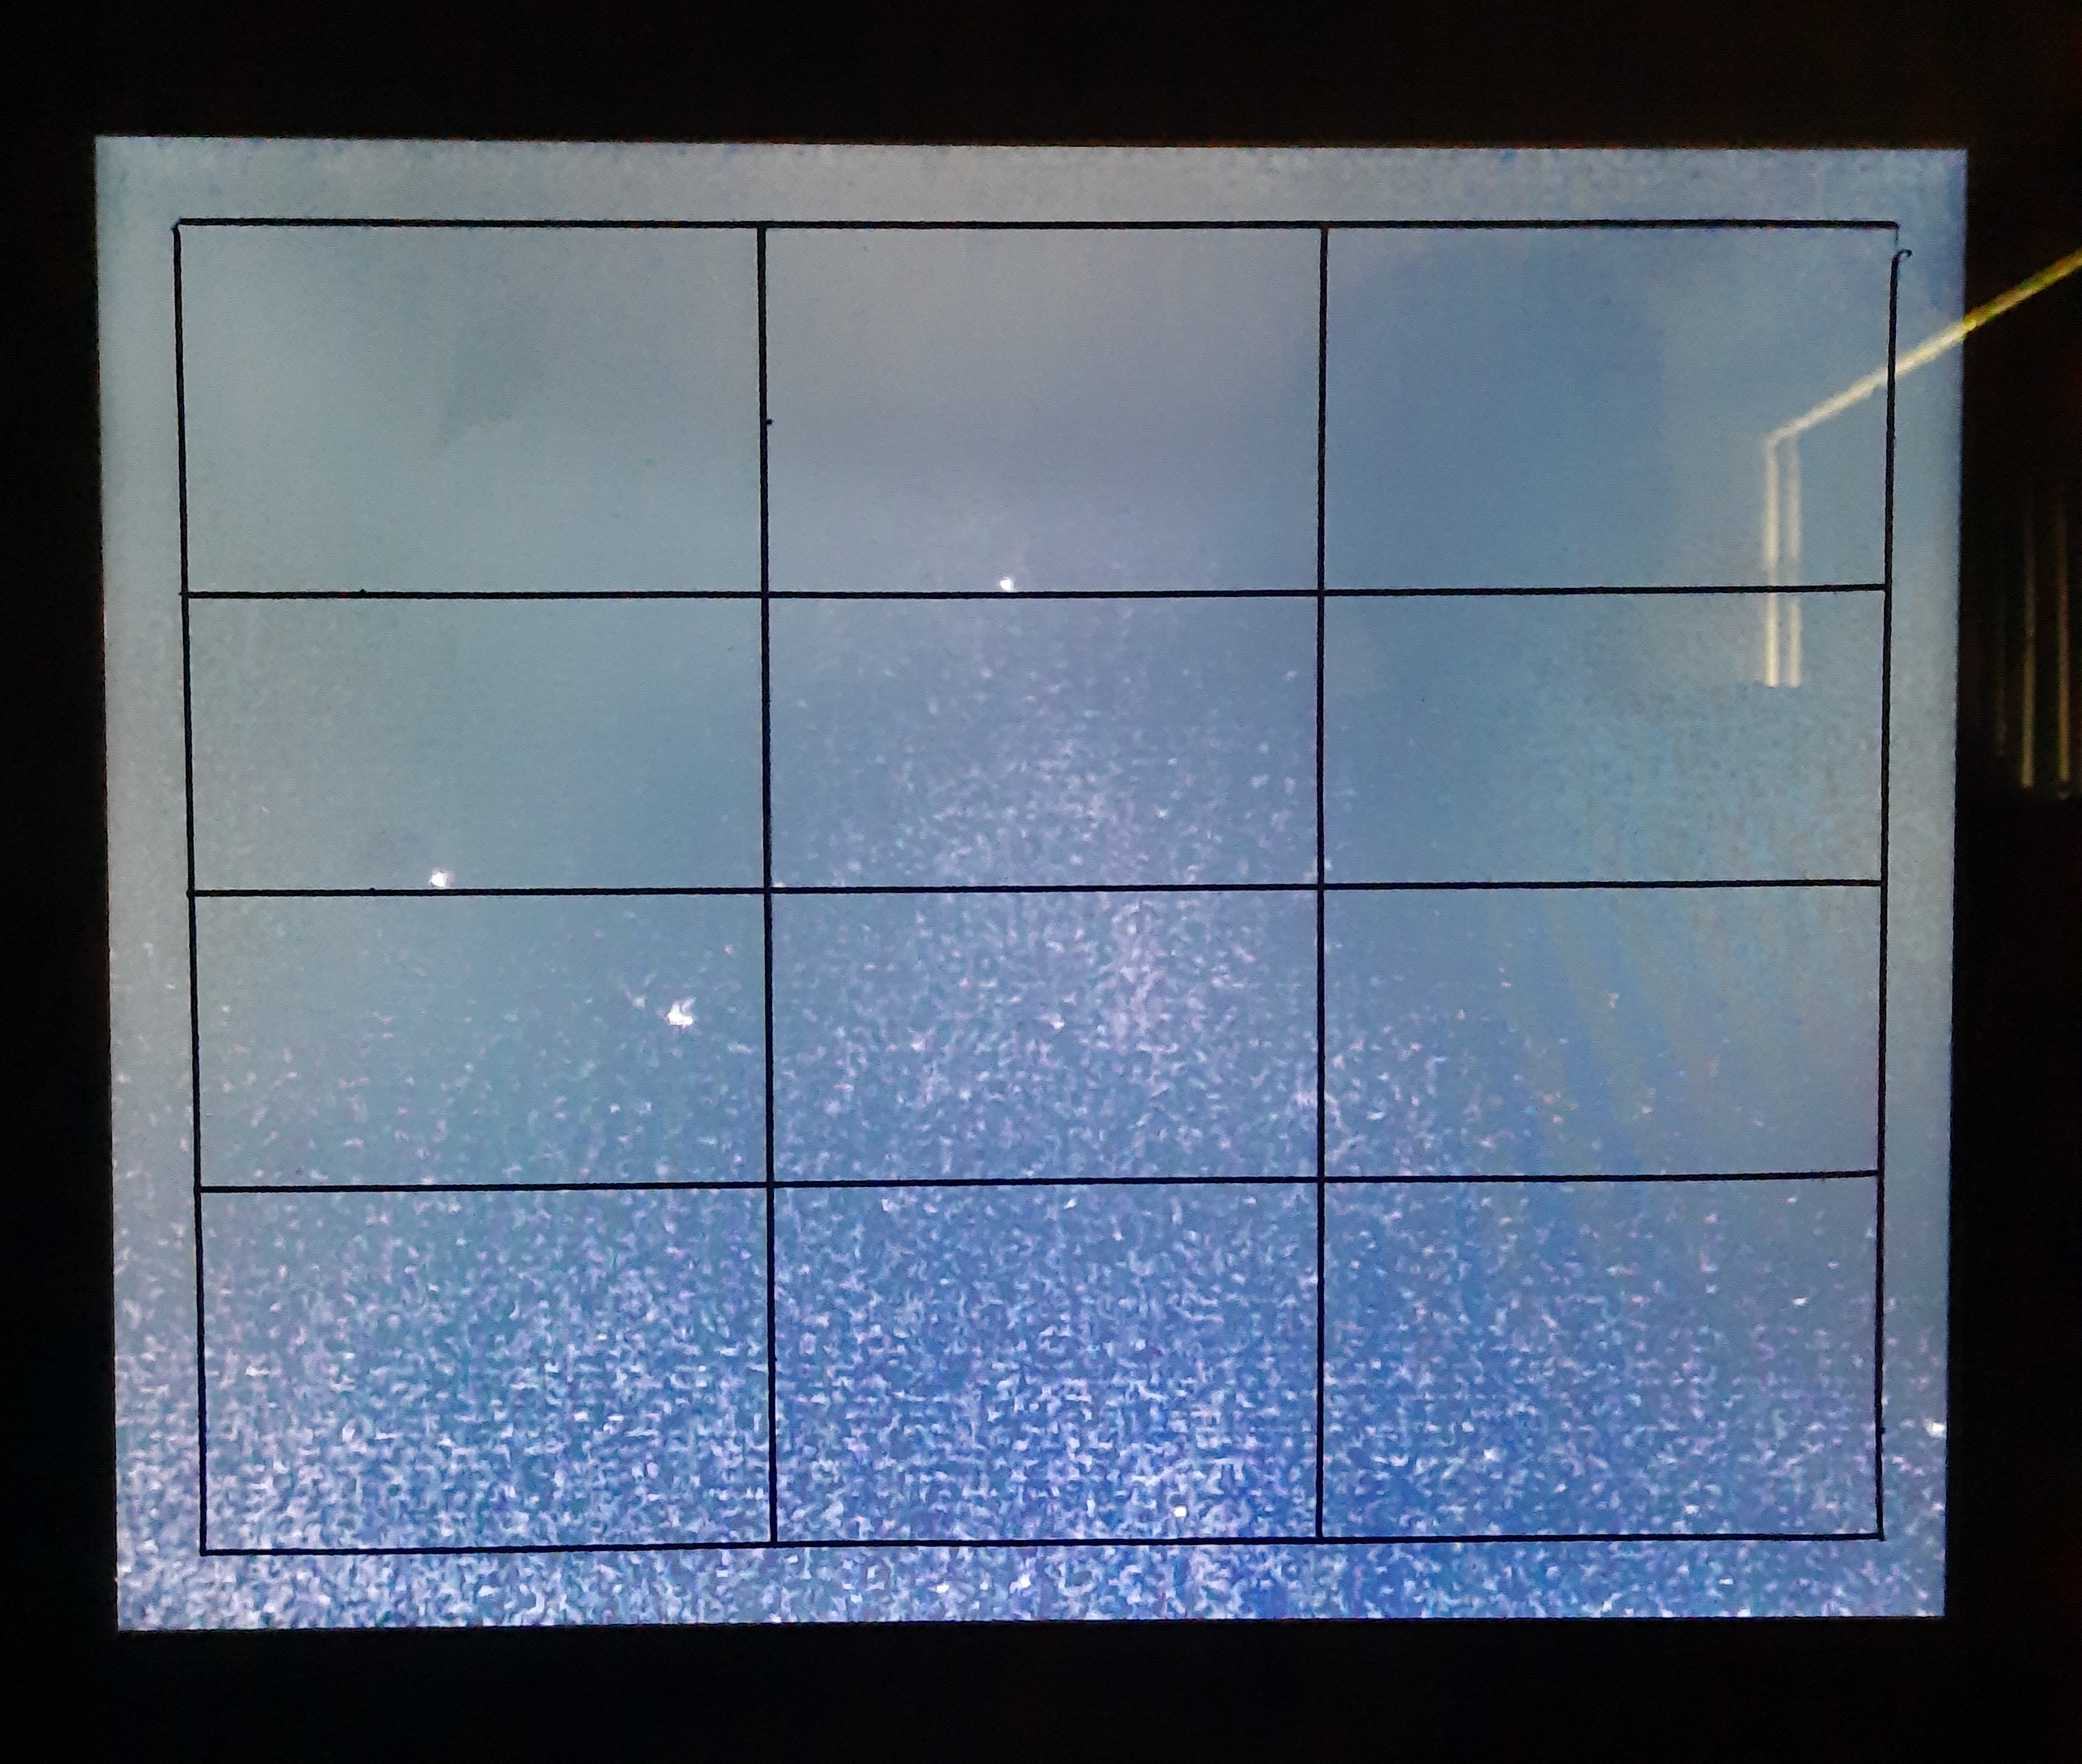
\includegraphics[width=8.3cm,height=4.5cm]{2} 
	\caption{Experimental setup in laboratory}
	\label{}
\end{figure}

\subsection{Precautions}
\begin{enumerate}
	\item {Always allow sufficient time for lamp to glow before taking readings}
	\item {Do not place hands near the lamp source. It is very hot. }
	\item {Do not touch optical surfaces with fingers.}
	\item {Switch off the power supply before making any changes.}
\end{enumerate}


\section{Observation and Analysis}
\begin{figure}[H] %  figure placement: here, top, bottom, or page
	\centering
	\includegraphics[width=8.3cm,height=6cm]{3} 
	\caption{Calibration curve for magnetic pole pieces.}
	\label{3}
\end{figure}

\begin{figure}[H] %  figure placement: here, top, bottom, or page
	\centering
	\includegraphics[width=8.3cm,height=6cm]{4} 
	\caption{Normal Zeeman effect}
	\label{4}
\end{figure}

\begin{figure}[H] %  figure placement: here, top, bottom, or page
	\centering
	\includegraphics[width=8.3cm,height=6cm]{long} 
	\caption{Longitudinal Zeeman effect}
	\label{1}
\end{figure}

\begin{figure}[H] %  figure placement: here, top, bottom, or page
	\centering
	\includegraphics[width=8.3cm,height=6cm]{an} 
	\caption{Anomalous  Zeeman effect}
	\label{p}
\end{figure}

\begin{figure}[H] %  figure placement: here, top, bottom, or page
	\centering
	\includegraphics[width=8.3cm,height=6cm]{lwp} 
	\caption{Anomalous  Zeeman effect in longitudinal direction with polariser.}
	\label{ss}
\end{figure}

\begin{table}[H]
	\centering
	\caption{Table for measurement radius of lines}
	\label{tab:my-table}
	\resizebox{\columnwidth}{!}{%
		\begin{tabular}{|c|c|ccc|r|r|r|}
			\hline
			\multirow{2}{*}{Vernier Reading} &
			\multirow{2}{*}{Component} &
			\multicolumn{3}{c|}{Radius} &
			\multicolumn{1}{l|}{\multirow{2}{*}{$r_1^2$ ($\mu m^2$)}} &
			\multicolumn{1}{l|}{\multirow{2}{*}{$r_2^2$ ($\mu m^2$)}} &
			\multicolumn{1}{l|}{\multirow{2}{*}{$r_3^2$ ($\mu m^2$)}} \\ \cline{3-5}
			&
			&
			\multicolumn{1}{c|}{$r_1$ ($\mu m$)} &
			\multicolumn{1}{c|}{$r_2$ ($\mu m$)} &
			$r_3$ ($\mu m$) &
			\multicolumn{1}{l|}{} &
			\multicolumn{1}{l|}{} &
			\multicolumn{1}{l|}{} \\ \hline
			\multirow{2}{*}{41} & $\sigma_+$ & \multicolumn{1}{c|}{2998.88} & \multicolumn{1}{c|}{4921.58} & 6226.76 & 8993281.254 & 24221949.7  & 38772540.1  \\ \cline{2-8} 
			& $\sigma_-$ & \multicolumn{1}{c|}{1214.09} & \multicolumn{1}{c|}{4155.9}  & 5677.94 & 1474014.528 & 17271504.81 & 32239002.64 \\ \hline
			\multirow{2}{*}{42} & $\sigma_+$ & \multicolumn{1}{c|}{2990.25} & \multicolumn{1}{c|}{4971.72} & 6259.09 & 8941595.063 & 24717999.76 & 39176207.63 \\ \cline{2-8} 
			& $\sigma_-$ & \multicolumn{1}{c|}{1517.98} & \multicolumn{1}{c|}{4249.52} & 5715.25 & 2304263.28  & 18058420.23 & 32664082.56 \\ \hline
			\multirow{2}{*}{44} & $\sigma_+$ & \multicolumn{1}{c|}{2983.79} & \multicolumn{1}{c|}{4948.42} & 6187.39 & 8903002.764 & 24486860.5  & 38283795.01 \\ \cline{2-8} 
			& $\sigma_-$ & \multicolumn{1}{c|}{1893.39} & \multicolumn{1}{c|}{4362.2}  & 5841.22 & 3584925.692 & 19028788.84 & 34119851.09 \\ \hline
			\multirow{2}{*}{45} & $\sigma_+$ & \multicolumn{1}{c|}{2986.57} & \multicolumn{1}{c|}{4917.36} & 6213.49 & 8919600.365 & 24180429.37 & 38607457.98 \\ \cline{2-8} 
			& $\sigma_-$ & \multicolumn{1}{c|}{1996.95} & \multicolumn{1}{c|}{4432.3}  & 5862.09 & 3987809.303 & 19645283.29 & 34364099.17 \\ \hline
		\end{tabular}%
	}
\end{table}

\begin{figure}[H] %  figure placement: here, top, bottom, or page
	\centering
	\includegraphics[width=8.3cm,height=6.5cm]{pl} 
	\caption{Plot of wave number versus magnetic field}
\end{figure}

\begin{table}[H]
	\centering
	\caption{Calculation of Delta}
	\resizebox{\columnwidth}{!}{%
		\begin{tabular}{|c|ccc|c|}
			\hline
			\multirow{2}{*}{Vernier Reading} & \multicolumn{3}{c|}{$\delta$ ($\mu m^2$)} & \multirow{2}{*}{$\delta$} \\ \cline{2-4}
			& \multicolumn{1}{c|}{$\delta^1$}  & \multicolumn{1}{c|}{$\delta^2$}  & $\delta^3$  &             \\ \hline
			41 & \multicolumn{1}{c|}{7519266.726} & \multicolumn{1}{c|}{6950444.886} & 6533537.454 & 7001083.022 \\ \hline
			42 & \multicolumn{1}{c|}{6637331.782} & \multicolumn{1}{c|}{6659579.528} & 6512125.066 & 6603012.125 \\ \hline
			44 & \multicolumn{1}{c|}{5318077.072} & \multicolumn{1}{c|}{5458071.656} & 4163943.924 & 4980030.884 \\ \hline
			45 & \multicolumn{1}{c|}{4931791.062} & \multicolumn{1}{c|}{4535146.08}  & 4243358.812 & 4570098.651 \\ \hline
		\end{tabular}%
	}
\end{table}

% Please add the following required packages to your document preamble:
% \usepackage{multirow}
% \usepackage{graphicx}
\begin{table}[H]
	\centering
	\caption{Calculation of $\Delta \nu$ and Calibration of pole pieces.}
	\resizebox{\columnwidth}{!}{%
		\begin{tabular}{|c|c|c|cc|c|r|}
			\hline
			\multirow{2}{*}{Vernier Reading} &
			\multirow{2}{*}{$B$ ($T$)} &
			\multirow{2}{*}{Component} &
			\multicolumn{2}{c|}{$\Delta$ ($\mu m^2$)} &
			\multirow{2}{*}{$\Delta$} &
			\multicolumn{1}{c|}{\multirow{2}{*}{$\Delta \nu$ ($m^{-1}$)}} \\ \cline{4-5}
			&
			&
			&
			\multicolumn{1}{c|}{$\Delta^{2,\,1}$} &
			$\Delta^{3,\,2}$ &
			&
			\multicolumn{1}{c|}{} \\ \hline
			\multirow{2}{*}{41} &
			\multirow{2}{*}{0.515} &
			$\sigma_+$ &
			\multicolumn{1}{c|}{15228668.44} &
			14550590.4 &
			\multirow{2}{*}{15136061.74} &
			\multirow{2}{*}{50.0587921} \\ \cline{3-5}
			&
			&
			$\sigma_-$ &
			\multicolumn{1}{c|}{15797490.28} &
			14967497.83 &
			&
			\\ \hline
			\multirow{2}{*}{42} &
			\multirow{2}{*}{0.45} &
			$\sigma_+$ &
			\multicolumn{1}{c|}{15776404.7} &
			14458207.87 &
			\multirow{2}{*}{15148607.96} &
			\multirow{2}{*}{47.21252557} \\ \cline{3-5}
			&
			&
			$\sigma_-$ &
			\multicolumn{1}{c|}{15754156.95} &
			14605662.33 &
			&
			\\ \hline
			\multirow{2}{*}{44} &
			\multirow{2}{*}{0.365} &
			$\sigma_+$ &
			\multicolumn{1}{c|}{15583857.73} &
			13796934.52 &
			\multirow{2}{*}{14978929.41} &
			\multirow{2}{*}{35.60796663} \\ \cline{3-5}
			&
			&
			$\sigma_-$ &
			\multicolumn{1}{c|}{15443863.15} &
			15091062.25 &
			&
			\\ \hline
			\multirow{2}{*}{45} &
			\multirow{2}{*}{0.325} &
			$\sigma_+$ &
			\multicolumn{1}{c|}{15260829} &
			14427028.61 &
			\multirow{2}{*}{15016036.87} &
			\multirow{2}{*}{32.67688978} \\ \cline{3-5}
			&
			&
			$\sigma_-$ &
			\multicolumn{1}{c|}{15657473.99} &
			14718815.88 &
			&
			\\ \hline
		\end{tabular}%
	}
\end{table}

From this plot we obtain the slope as $98.26\pm13.31$ $(mT)^{-1}$. With the slope obtained we use equation (8), to obtain Bohr's magneton as $(9.76\pm1.32)\times10^{-24}  JT^{-1}$ . The error can be calculated as

\begin{equation}
	\frac{\delta \mu_B}{\mu_B}=\frac{\delta m}{m}
\end{equation}

where m is slope, $\delta$ is associated error of that quantity. 

The literature value of Bohr's magneton is $9.27\times10^{-24} $ $JT^{-1}$ with the relative error is 4.97 \%

\section{Conclusion and Summary}
Zeeman effect is splitting of spectral lines under time independent magnetic field, due to interaction between the magnetic field and the spin angular momentum of the electrons where each of the electrons has its spin. Fabry Perot etalon was used to observed spectral lines. With the magnetic field turned on in the absence of the analyser three lines can be seen simultaneously in the normal Zeeman effect in transversal observation. In the case of the anomalous Zeeman effect three groups of three lines appear. The various Zeeman efffects with polariser was studied. We obtained Bohr Magneton's value $(9.76\pm1.32)\times10^{-24}  JT^{-1}$ with the relative error as  4.97 \%.  

The error can be reduced by properly adjusting the distance of lenses, camera and etalon such that the lines are visible sharp to facilitate the determination of radius. The apparatus should be in ambient temperature to avoid optical error artifacts.  Random errors and human errors may also have contributed. 

\section{References}
\begin{enumerate}
	\item {\url{https://www.niser.ac.in/sps/sites/default/files/basic_page/Zeemaneffect-manual.pdf}}
	\item {Zeeman effect old manual SPS NISER}
	\item {\url{https://en.wikipedia.org/wiki/Fabry%E2%80%93P%C3%A9rot_interferometer}}
	\item {\url{https://www.nikhef.nl/~h73/kn1c/praktikum/phywe/LEP/Experim/5_1_10.pdf}}
\end{enumerate}

\end{document}